\chapter{Asking Dubai Billionaires How They Got Rich}

This lecture begins by spending scale before it spends explanation. We are shown yachts, Rolls-Royces, and yearly money claims large enough to force the question, and only then does the host reset the frame and begin the real inquiry. From that point forward the episode unfolds in a clear order: risk first, then pivot and sales, then real-estate entry arithmetic, then developer-scale branding and focus, and finally the belief that keeps the operator moving when calculation alone no longer feels sufficient.

\begin{remark}
No validated mathematical board frame survives for this lecture. Accordingly, the displayed relations below are either transcript-backed extractions or cautious reconstructions from the spoken sequence. Likewise, the quoted ``most amount of money in a single year'' figures are preserved as scale claims, without pretending that the lecture audits whether each number is revenue, profit, or some broader business total.
\end{remark}

\section{Cold Open and the Dubai Field Site}

The first forty seconds are not yet a stable argument. They are a promise reel. We see a yacht, the claim of a cannabis billionaire, a man with six Rolls-Royces, and gigantic one-year money numbers. The function of this splice is simple: it creates pressure around one governing question. What mechanism sits underneath these visible markers of wealth?

That pressure is then stabilized by the host's reset. We are in Dubai; we are going to the wealthiest parts of the city; and the purpose is to interview millionaires and billionaires in order to figure out how they built wealth and how some version of their method might be copied. In other words, the lecture turns spectacle into fieldwork.

It is useful to compress the opening challenge into one schematic line:
\begin{equation}
\text{visible wealth} \to \text{hidden mechanism?}
\end{equation}
The rest of the chapter fills in the right-hand side, one interview at a time.

\section{Cannabis, Risk, and Leverage}

The first stable interview stays with the cannabis entrepreneur. The lecture establishes scale first, as it often does:
\begin{equation}
Y_{\text{cannabis}} \approx 1\,\text{billion euros/year}.
\end{equation}
But that number is only the outer shell. The host immediately asks for the best financial advice behind it, and the answer is a father's rule, stated in pounds but better kept in the transcript's simple operator form:
\begin{equation}
10 \to 20,
\qquad
\text{because }10\text{ can be earned again.}
\end{equation}
We should not over-refine this into formal finance. The lecture's point is narrower and sharper:
\begin{equation}
\text{recoverable downside} \to \text{willingness to risk for larger upside}.
\end{equation}

The next beat is important for motivation. The biggest risk was not a familiar extension of prior expertise. The speaker says he had been in the nightclub business and then entered cannabis without really knowing that industry. The lecture wants us to see that the risk rule is not decorative. It is the thing that licenses a move into the unknown.

Scale is then immediately paired with vulnerability. The guest says he had been broke several times, including during the Cyprus banking crisis. That sets up one of the chapter's cleanest cautionary claims:
\begin{equation}
\text{money in the bank} \neq \text{money under direct control}.
\end{equation}
A cautious reconstruction, no more than that, is
\begin{equation}
D_{\text{customer}} \mapsto L_{\text{bank}},
\end{equation}
so that what appears as ``my money in the bank'' is really a claim on an institution. The lecture does not give a banking theory, but it does insist on this difference between apparent possession and direct control.

The interview then makes a quick detour through formal education. The guest says he was expelled from school at thirteen and never went back. The host's follow-up is exactly right for the lecture's structure: if university is not the source here, then what lesson about business replaces it? The answer is not a spreadsheet. It is social environment:
\begin{equation}
n_{\text{drunks}}=5 \to \text{you become the 6th drunk},
\qquad
n_{\text{billionaires}}=5 \to \text{you become the 6th billionaire}.
\end{equation}
Or, in a cleaner form,
\begin{equation}
\text{peer group} \to \text{behavioral drift} \to \text{identity outcome}.
\end{equation}

Only after that does the lecture ask what distinguishes billionaires from millionaires. The answer is motivational rather than merely numerical:
\begin{equation}
\text{work} \to \text{success},
\qquad
\text{not primarily } \text{work} \to \text{money}.
\end{equation}
This sits next to another claim of rebuild confidence. If stripped of everything, the operator says he could still return. The language is theatrical, but the point is plain: money is not the deepest asset if the operating pattern remains intact.

That sets up the final line of the interview, which the host very wisely recaps instead of leaving as mere attitude. ``Don't negotiate'' becomes, in the host's translation, a doctrine of leverage:
\begin{equation}
\text{leverage}\uparrow \to \text{need to negotiate}\downarrow,
\qquad
\text{walk-away power}\uparrow.
\end{equation}
The lecture has now moved from risk, to loss, to social environment, to negotiation, and that sequence matters. Walk-away power only makes sense after we understand why the operator believes he can survive the absence of a deal.

\subsection{Question \& Answer}

\paragraph{Question.} What changes when leverage is strong enough that one can walk away instead of negotiate?

\paragraph{Answer.} The lecture's answer is that bargaining stops being the center of the scene. Once the operator does not need this particular deal in order to remain alive, the transaction must fit him rather than rescue him. ``My way or the highway'' is therefore not only temperament. It is the surface expression of independence from the immediate deal.

\section{Yacht Wealth and the COVID Pivot}

The lecture then changes scene on purpose. We go to Dubai Harbor, where the host stops talking about billionaire identity in the abstract and starts asking how visible luxury assets are financed in practice. The next interview begins with business count and duration: eight businesses, twenty-two years. Only then does it ask for the decisive scaling story.

Here the spoken scale markers are
\begin{align}
R_{\text{pre-pivot}} &\approx \$10\,\text{million}, \\
R_{\text{pivot-year}} &\approx \$69\,\text{million}, \\
R_{\text{core,later}} &\approx \$35\,\text{million}.
\end{align}
The lecture's rhythm is especially good here. First the host frames the jump from roughly ten million to sixty-nine million. Then the guest gives us the historical shock that made the jump necessary: COVID arrived, exhibitions closed, promotional products stalled, and the original business plummeted.

The recovery does not come from optimism alone. It comes from a usable chain: family background in healthcare, a decade of operational knowledge in China, and direct contact with hospitals. In the notes we can preserve that mechanism as
\begin{equation}
\text{promotional products crash}
\to
\text{medical supplies pivot}
\to
\text{direct hospital sales}
\to
R_{\text{pivot-year}}.
\end{equation}

\begin{figure}[h]
\centering
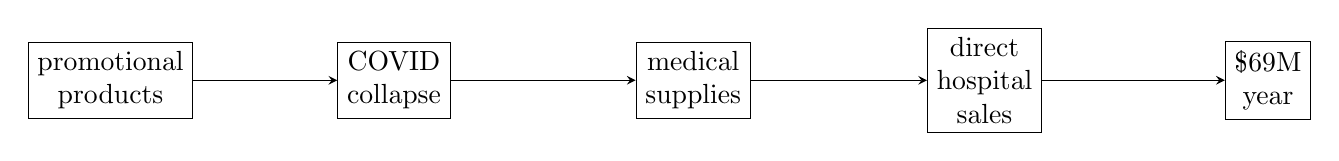
\begin{tikzpicture}[>=stealth]
\node[draw, align=center] (a) at (0,0) {promotional\\products};
\node[draw, align=center] (b) at (3.6,0) {COVID\\collapse};
\node[draw, align=center] (c) at (7.4,0) {medical\\supplies};
\node[draw, align=center] (d) at (11.1,0) {direct\\hospital\\sales};
\node[draw, align=center] (e) at (14.7,0) {\$69M\\year};

\draw[->] (a) -- (b);
\draw[->] (b) -- (c);
\draw[->] (c) -- (d);
\draw[->] (d) -- (e);
\end{tikzpicture}
\caption{Transcript-led reconstruction of the pivot chain described in the harbor interview.}
\end{figure}

There is also a small numerical tension here, and the notes should keep it visible. If we compute the host-framed jump directly, we get
\begin{equation}
g_{\text{pivot}}
=
\frac{R_{\text{pivot-year}}}{R_{\text{pre-pivot}}}
\approx
\frac{69}{10}
\approx 6.9.
\end{equation}
But the guest later says they had ``5x the business before.'' The right move is not to force agreement. It is to preserve both spoken claims and let the reader see that the lecture is giving us business arithmetic in the register of remembered operator speech, not audited financial statements.

\subsection{Question \& Answer}

\paragraph{Question.} How do we pivot when the original business collapses?

\paragraph{Answer.} The lecture's answer is concrete: a pivot requires a new urgent product, an already available operational competence, and a sales route that reaches the buyer without delay. Crisis is only the pressure. The actual pivot is the new chain that converts pressure into orders.

\section{Sales as Question-Removal Rather Than Pressure}

Once the pivot has been explained, the lecture does not leave the matter at ``we adapted.'' It asks what practical faculty made the adaptation work. The answer is selling, and the guest states the permanence of the claim in almost liturgical form:
\begin{equation}
\text{selling was key before},
\quad
\text{selling is key today},
\quad
\text{selling will be key in the future}.
\end{equation}
This is not filler. It is the point at which the lecture turns from story into method.

The core sales model is likewise simple enough to write down:
\begin{equation}
Q\uparrow \to O\downarrow \to P(\text{close})\uparrow,
\end{equation}
where \(Q\) denotes useful questioning, \(O\) unresolved objections, and \(P(\text{close})\) the probability of closing. The guest's language is deliberately strong: ask so many questions that the customer would be foolish not to buy. But what matters is the mechanism. Questions are not stage business. They are an instrument for locating what is still unclear.

That is why the underrated closing question is so good. ``What did you like most about my presentation?'' compels the buyer to articulate value in his own language. The follow-up, ``what else?,'' keeps drawing out the structure of assent until the unresolved remainder is small.

The lecture then adds a second piece that is more operational than moral. Making payment easy is part of the close:
\begin{equation}
p_{\text{card XYZ}} \approx 0.8,
\qquad
\text{payment friction}\downarrow \to P(\text{pay})\uparrow.
\end{equation}
One can think of this as the final stage of objection removal. Even if the desire is present, awkward payment mechanics can still destroy the close.

The harbor interview also folds trust into the same mechanism. Nice questioning, relation-building, and trust-building are not alternatives to selling. They are the means by which unresolved resistance is reduced.

\subsection{Question \& Answer}

\paragraph{Question.} What question actually moves a sale toward closure?

\paragraph{Answer.} In the lecture, the decisive question is the one that makes the buyer explain the attraction of the offer back to himself. ``What did you like most?'' is powerful because it turns the customer's own words into the first draft of the close. The salesperson then keeps asking until the remaining objections have no place left to hide.

\section{Mindset, Self-Talk, and the Harbor Recap}

The harbor interview then widens from selling to entrepreneurial interiority. The book named is \emph{Think and Grow Rich}, but the lecture preserves the lesson in a more compressed form:
\begin{equation}
S_{\text{entrepreneurship}} \approx 0.9\,\text{mindset}+0.1\,\text{financial technique}.
\end{equation}
This is clearly a heuristic rather than a measurement, but we should keep its function. It explains why the lecture moves from closing mechanics to belief without treating that move as a change of subject.

The same structure appears again in the self-talk doctrine:
\begin{equation}
\text{words to oneself} \to \text{subconscious response} \to \text{action}.
\end{equation}
The claim is that the mind follows repeated verbal direction. Even when the operator feels weak, he is told to speak strength; even when he feels unwell, he is told to speak health. The point is not psychological elegance. The point is operational alignment between inner language and outer action.

This section also contains the harbor interview's explicit movement toward faith: hope as the last resort of humanity, and not believing in oneself as a kind of refusal of possibility. The host's recap then condenses the entire sequence into a line that matters for the logic of the chapter: believing that one can is more profitable than believing that one cannot. That recap is important because it translates personal philosophy back into business consequence.

\section{Real Estate Without Starting Capital}

The next interview begins, quite characteristically, with visible scale once again: a Rolls-Royce, six of them in fact, and a one-year money claim in real estate:
\begin{equation}
Y_{\text{real-estate}} \approx 10\,\text{billion dirhams/year}.
\end{equation}
Only then does the lecture ask the more useful question. Must one come from money in order to become a billionaire? The answer is a flat no, followed by the headline statistic
\begin{equation}
p_{\text{first-gen billionaires}} \approx 0.85.
\end{equation}
The garbled follow-up percentage about the second generation should not be forced into precision. The chapter should preserve the stronger point instead: the lecture wants to remove inheritance as an excuse before it offers an entry mechanism.

That mechanism is brokerage. The real-estate arithmetic is the cleanest in the whole episode:
\begin{align}
c_{\text{broker}} &= 5\%, \\
V &= 10\,\text{million AED}, \\
c_{\text{broker}}V &= 0.5\,\text{million AED}.
\end{align}
It is worth showing the calculation in the plainest possible way.

\paragraph{Worked Example.}
\begin{enumerate}
\item Take the spoken commission rate \(c_{\text{broker}}=5\%=0.05\).
\item Take the transaction value \(V=10{,}000{,}000\ \text{AED}\).
\item Multiply:
\[
0.05 \times 10{,}000{,}000 = 500{,}000.
\]
\item Therefore
\[
c_{\text{broker}}V = 500{,}000\ \text{AED} = 0.5\,\text{million AED}.
\]
\end{enumerate}

The lecture's ladder is then immediate:
\begin{equation}
\text{brokerage} \to \text{developer}.
\end{equation}
One does not begin by owning the tower. One begins by participating in the transaction flow that surrounds the tower.

This interview then returns to selling, but now in a more contradictory and therefore more interesting way. The guest says salesmanship is an inborn quality, something not everybody can become. Yet almost at once he teaches a process: listen to the customer's requirement, understand budget, distinguish luxury from affordability, explain benefits, and make the return legible. The notes should preserve that tension rather than smooth it away. The lecture itself does not resolve it. It simply allows both claims to stand.

A compact formalization of the teachable part is
\begin{equation}
\text{buyer need} + \text{budget fit} + \text{ROI clarity}
\to
P(\text{purchase})\uparrow.
\end{equation}
The transcript's English is rough when it speaks about how fast the buyer makes his money back or doubles it, but the business content is clear enough: payback speed and upside visibility help close the deal.

\subsection{Question \& Answer}

\paragraph{Question.} How can somebody start creating wealth in real estate today if he does not begin with capital?

\paragraph{Answer.} The lecture's answer is to begin where deal size already exists but ownership is not yet required. Brokerage lets us participate in large asset transfers through commission rather than starting balance sheet. The path is therefore not magic. It is sequential: distribution first, accumulation second, development third.

\section{Product-as-Billboard, One Core, and Faith}

After a sponsor-style hinge, the lecture returns at its highest altitude. The final guest is a property developer behind branded residences, and the sequence again begins with scale:
\begin{equation}
Y_{\text{developer}} \approx \$5\,\text{billion}/\text{year}.
\end{equation}
The first answer is blunt: sales and marketing are everything. But the lecture does not stop at the familiar phrase. It asks what kind of marketing scales, especially when early resources are thin. The answer is omnipresence:
\begin{equation}
\text{marketing} \to \text{omnipresence}.
\end{equation}

The interesting move comes next. Omnipresence is not achieved here only by buying media. It is pursued by making the product recognizable enough to advertise itself:
\begin{equation}
\text{architectural DNA}
\to
\text{recognizability}
\to
\text{self-marketing product}.
\end{equation}
The buildings become the billboards. The developer does not merely place a brand on the product; he designs the product so that the brand is legible in the form itself.

\begin{figure}[h]
\centering
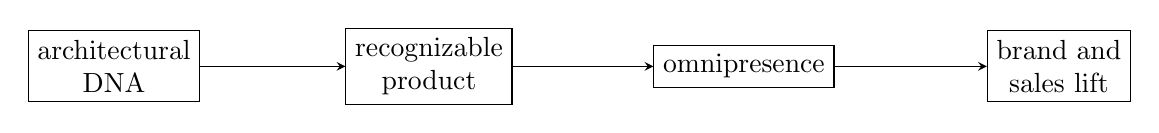
\begin{tikzpicture}[>=stealth]
\node[draw, align=center] (a) at (0,0) {architectural\\DNA};
\node[draw, align=center] (b) at (4.0,0) {recognizable\\product};
\node[draw, align=center] (c) at (8.0,0) {omnipresence};
\node[draw, align=center] (d) at (12.0,0) {brand and\\sales lift};

\draw[->] (a) -- (b);
\draw[->] (b) -- (c);
\draw[->] (c) -- (d);
\end{tikzpicture}
\caption{Transcript-led reconstruction of the product-as-billboard strategy described in the final interview.}
\end{figure}

Only after this marketing architecture is established does the lecture move to focus. The guest says that diversification across unrelated sectors had been one of his mistakes. The better lesson was to remain inside one core and widen there:
\begin{equation}
\text{one core} \to \text{multiple product lines within the core} \to \text{scale}.
\end{equation}
The examples are all intra-core: luxury real estate, mid-market real estate, lower-end real estate. The host glosses this as vertical integration:
\begin{equation}
\text{focus within one core} \approx \text{vertical integration}.
\end{equation}
That gloss is not exact in the strict industrial sense, but it captures the lecture's intended lesson well enough. The enemy here is scattered attention.

\subsection{Question \& Answer}

\paragraph{Question.} How can the product itself perform part of the marketing?

\paragraph{Answer.} The lecture's answer is that a product can carry a repeated grammar, so that recognition arrives before explanation. When the object is identifiable on sight, attention has already been captured and part of the marketing budget has effectively been moved into design.

The final movement then returns, once more, from method to belief. Faith is said to be everything. Miracles are mentioned without irony. The developer recounts a moment when he thought he had lost it all, asked God for a miracle, and moved from ``out of my hands'' to ``in your hands.'' The lecture does not mathematize this, and neither should we. Its role is different. It names the resource that remains when focus, product, and sales have been pushed as far as technique alone can push them.

\section{Summary}

The lecture begins with a montage and ends with a chain of operator rules. The order matters. First we are shown the surfaces of wealth. Then we are led through the mechanisms that claim to support them: risk on recoverable downside, caution about banked money, the pull of peer groups, the leverage of walking away, the necessity of pivot under pressure, the permanence of selling, the commission arithmetic of brokerage, the value of product recognizability, and the superiority of one deep core over scattered ambition.

In compressed form, the chapter leaves us with the following sequence:
\begin{align}
\text{recoverable downside} &\to \text{risk}, \\
\text{peer group} &\to \text{identity drift}, \\
\text{leverage}\uparrow &\to \text{negotiation need}\downarrow, \\
\text{collapse} &\to \text{pivot} \to \text{new channel}, \\
Q\uparrow &\to O\downarrow \to P(\text{close})\uparrow, \\
\text{brokerage} &\to \text{developer}, \\
\text{architectural DNA} &\to \text{recognizability} \to \text{omnipresence}, \\
\text{one core} &\to \text{scale}.
\end{align}
Read this way, the lecture is not a gallery of rich people. It is a staged inquiry into how risk appetite, sales process, transactional arithmetic, brand form, and sustaining belief are made to cooperate inside a commercial life.